\chapter{Review: Diffusion Models}
\label{sec:diffusion}

Diffusion models, or DMs~\citep{sohl2015deep,ho2020denoising,nichol2021improved,song2020score}, can be understood as hierarchical variational auto-encoders with a very simple encoder: rather than parameterising a distribution with a neural network, the encoder simply adds Gaussian noise to the data. This ``encoder'' is commonly then referred to as the ``forward'' (or ``noising'') process. The equivalent of the VAE's prior and decoder are then the ``reverse'' (or ``generative'') process, which uses a learned ``denoising'' function in the form of a neural network. Sampling from a DM begins with drawing a sample from a Gaussian distribution that approximates a heavily noised sample from the data distribution. Running the reverse/generative process on this sample then gradually removes noise from it, moving the sample closer to the data manifold. By the end of the generative process, if all is trained well, the samples from this process should match the data distribution. As we will show later, fitting the DM simply involves training a neural network to predict clean data give noisy data using a mean-squared error loss. This leads to more stable training than for a VAE, in which the prior, decoder, and encoder are all learned jointly, leading to a ``moving target'' problem as each component must keep compensating for changes to the others.

\begin{figure}
    \centering
    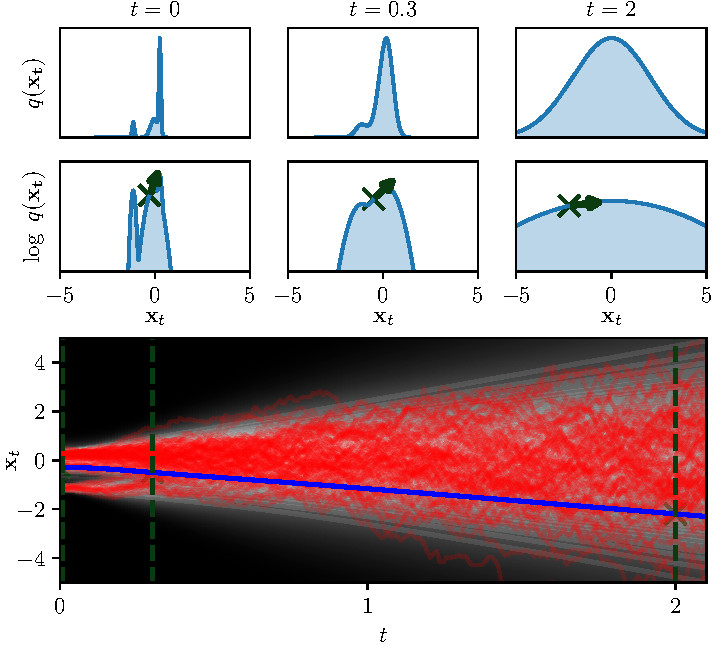
\includegraphics[scale=1]{figs/thesis/diffusion_process.pdf}
    \caption{An example diffusion process for the data distribution $q(\rvx_0)$ shown at the top left. We use $g(t) := \sqrt{2t}$ so that $\sigma_t = t$. \textbf{Top row:} The data distribution $q(\rvx_0)$ and marginals $q(\rvx_t)$ for $t=0.3$ and $t=2$. These marginals are the convolution of the data distribution with a Gaussian distribution of standard deviation $\sigma = t$. For $t=2$, the distribution looks near-Gaussian. \textbf{Middle row:} The distributions from the top row shown in log-space. The green tangent arrows represent $\nabla_{\rvx_t} \log q(\rvx_t)$, the score functions that a neural network would be trained to estimate. \textbf{Bottom row:} The continuous evolution of the forward process for all $t$ between $0$ and $2$. The marginals plotted in the top rows correspond to the ``slices'' made by the dashed green lines. Each faded white line marks a percentile of the $q(\rvx_t)$. The red lines are stochastic trajectories sampled with the SDE described in \cref{sec:diffusion-forward-sde}. The blue line is sampled with the ODE described in \cref{sec:diffusion-forward-ode} and parameterized with the score estimates from the second row.}
    \label{fig:diffusion-overview}
\end{figure}

\section{The forward process as an SDE} \label{sec:diffusion-forward-sde}
This forward process is defined through a combination of the initial condition $\rvx_0 \sim \pdata(\cdot|\rvy)$ and the stochastic differential equation (SDE):\footnote{We describe here the ``variance-exploding'' diffusion process. We generalise to a broader family of forward processes in ..., which require more complex notation.}
\begin{equation} \label{eq:forward-diffusion}
    \mathrm{d}\rvx = g(t) \mathrm{d}\rvw
\end{equation}
defined for all $t \geq 0$, with $\rvw$ being the standard Wiener process, also known as Brownian motion. The rate at which noise is added, $g(t)$, is a hyperparameter. We will keep this exposition general by not assuming any value for it, but note that \citet{karras2022elucidating} show that setting $g(t) := \sqrt{2t}$ yields good performance.

For any finite set of times $t_1,\ldots,t_n$, the forward process defines a joint distribution over all of $\rvx_{t_1},\ldots,\rvx_{t_n}$ and $\rvy$. We will denote such joint distributions as $q(\rvx_{t_1},\ldots,\rvx_{t_n}, \rvy)$, and similarly denote marginal or conditional distributions derived from them with $q$, with the specific distribution of interest being clear from variable names. In this notation, $q(\rvx_0,\rvy) = \pdata(\rvx_0,\rvy)$ is the data distribution. Many conditional distributions that follow from this are tractable, including the distribution over a variable at time $t$ conditioned on its value at time $0$:
\begin{equation}
    q(\rvx_t|\rvx_0,\rvy) := \gN \left( \rvx_t; \rvx_0, \sigma_t^2 \mI \right) \quad \text{where} \quad \sigma_t^2 := \int_0^t g(t')^2 \mathrm{d}t'.
\end{equation}
If we view the forward process as adding noise to clean data then $\sigma_t$ can be viewed as the ``noise-to-signal ratio'' of $\rvx_t$ and, if we follow \citet{karras2022elucidating} by setting $g(t) := \sqrt{2t}$ then we have the simple relationship that $\sigma_t = t$ for all $t\geq0$.

If $t$ is large and correspondingly $\sigma_t$ is large, $q(\rvx_t|\rvx_0,\rvy)$ will be very well approximated by the Gaussian $\gN(0; \sigma_t^2\mI)$. In particular, we can observe that the KL divergence
\begin{equation}
    \kl{q(\rvx_t|\rvx_0,\rvy)}{\gN(0; \sigma_t^2\mI)} :=\frac{1}{2\sigma_t^2} \rvx^\top \rvx
\end{equation}
diminishes with $\sigma_t^2$. This forward process can therefore be used to map from clean data $\rvx_0$ to data that is arbitrarily well-approximated by a simple distribution. In the next section we will discuss how to do the more challenging counterpart: transforming samples from a simple distribution into samples from the data distribution.

\section{The reverse SDE} \label{sec:diffusion-forward-sde}
Our aim in this section is to ``invert'' the forward process from the previous section, yielding a way to create clean data from noise. To do so we refer to a result  derived by \citet{anderson1982reverse}, and recalled in the diffusion modelling context by \citet{song2020score}, showing that the reverse of a diffusion process is also a diffusion process. A straightforward application of this result to the diffusion SDE in \cref{eq:forward-diffusion} reveals that the corresponding reverse-time diffusion SDE is
\begin{equation} \label{eq:reverse-diffusion}
    \mathrm{d}\rvx = -g(t)^2 \nabla_\rvx \log q(\rvx_t|\rvy) \mathrm{d}t + g(t) \mathrm{d}\bar{\rvw}
\end{equation}
with $\bar{\rvw}$ is a standard Wiener process when time flows backward from $\infty$ to $0$ and $\nabla_\rvx \log q(\rvx_t)$ is the generally intractable score of $q(\rvx_t)$ as defined through the forward process. The task of the neural network in a diffusion model is to estimate $\nabla_{\rvx_t} \log q(\rvx_t)$, and we will see in \cref{sec:diffusion-training} how this is done. Assuming that we have such an estimator, which we call $s_\theta(\rvx_t, \rvy, \sigma_t) \approx \nabla_{\rvx_t} \log q(\rvx_t)$, we can define a generative model as follows. Given large $T \in \mathbb{R}^{>0}$, we sample $\rvx_T \sim \gN(\vzero, \sigma_t^2 \mI)$; then we simulate the SDE
\begin{equation} \label{eq:reverse-diffusion-with-nn}
    \mathrm{d}\rvx = -g(t)^2 s_\theta(\rvx_t, \rvy, \sigma_t) \mathrm{d}t + g(t) \mathrm{d}\bar{\rvw}
\end{equation}
from time $t=T$ to $t=0$ with any SDE solver.\footnote{Possible choices include Euler integration~\citep{ho2020denoising}, more complex Runge-Kutta~\citep{grathwohl2018ffjord} solvers, or a Heun solver~\citep{karras2022elucidating}.} We will call the distribution over $\rvx_0$ parameterized by this process $p_\theta^\text{SDE}(\rvx_0)$. It approximates the data distribution $q(\rvx_0)$, with any approximation error being due to (1) imperfect fitting of the score function; and (2) the approximation of $q(\rvx_T)$ with a Gaussian. If $T$ is chosen to be large enough, source (1) will dominate. In practice there will also be some approximation error from numerically simulating the SDE, but we consider $p_\theta^\text{SDE}(\rvx_0)$ to be the distribution achieved with perfect SDE integration.

% Assuming that we have such an estimator, \cref{eq:reverse-diffusion} provides a way to morph from $\rvx_T$ sampled from a Gaussian distribution for some large $T$, to approximate samples from the data distribution $\rvx_0 \sim \pdata(\cdot|\rvy)$. To do so, we only need a tool for integrating SDEs. This can be simple like Euler integration, or may be a more complex Runge-Kutta~\citep{grathwohl2018ffjord} or Heun~\citep{karras2022elucidating} integration method.

\section{A reverse ODE} \label{sec:diffusion-ode}
In this section we will describe how to replace the SDE that parameterizes our generative model with an ODE. This can make the integration simpler and we will describe how it enables exact likelihood evaluation for any given $\rvx_0$.  \citet{song2020score} show that, for any diffusion process, there exists a deterministic process whose trajectories share the same marginal distributions $\{q(\rvx_t)\}_t$ as the stochastic diffusion process. This deterministic process is described by the ODE
\begin{align}
    \mathrm{d}\rvx &= - \frac{1}{2} g(t)^2 \nabla_\rvx \log q(\rvx_t|\rvy) \mathrm{d}t \\
    &\approx - \frac{1}{2} g(t)^2 \nabla_\rvx s_\theta(\rvx_t, \rvy, \sigma_t) \mathrm{d}t. \label{eq:diffusion-ode-with-nn}
\end{align}
We can now use the same generative model described in \cref{sec:diffusion-forward-sde} except that we integrate an ODE instead of an SDE. We will call the resulting distribution $p_\theta^\text{ODE}(\rvx_0)$. Note that this distribution will not necessarily be identical to $p_\theta^\text{SDE}(\rvx_0)$ if the approximation of the score function is imperfect, but both will approximate the data distribution.

Our now involves simply sampling $\rvx_T \sim \gN(\vzero, \sigma_t^2\mI)$ and then computing $\rvx_0 = f^{T:0}_\theta(\rvx_T)$, where $f^{T:0}_\theta$ is a function that simulates \cref{eq:diffusion-ode-with-nn} from time $T$ to $0$. Importantly, $f^{T:0}_\theta$ is deterministic and, since it comes from the integration of an ODE, invertible. If we assume that $f^{T:0}_\theta$ is also continuously differentiable then we can apply the change of variables rule to find
\begin{equation}
    p_\theta^\text{ODE}(\rvx_0) = p_\theta(\rvx_T) \left| \det \mJ_{f^{T:0}_\theta}(\rvx_T) \right|^{-1}
\end{equation}
where $\det \mJ_{f^{T:0}_\theta}(\rvx_T)$ is the determinant of the Jacobian of $f^{T:0}_\theta$ evaluated at $\rvx_T$. Following \citet{chen2018neural}, this can be efficiently estimated by integrating the trace
\begin{equation}
    \text{Tr}\left( \frac{\partial}{\partial \rvx_t} \left( - \frac{1}{2} g(t)^2 \nabla_\rvx s_\theta(\rvx_t, \rvy, \sigma_t) \right)
    \right)
\end{equation}
of the Jacobian of the ``drift'' term in \cref{eq:diffusion-ode-with-nn} along the path of $\rvx$ while simulating the ODE. \citet{song2020score} showed that diffusion models can yield statae-of-the-art data log likelihoods when evaluated in this way.

% A downside is that it has been observed empirically that not adding noise during integration can lead to more error build up if the approximation of $\nabla_\rvx \log q(\rvx_t|\rvy)$ is imperfect~\citep{karras2022elucidating}. We will describe in \cref{TODO} more advanced techniques which can combine the advantages of adding noise during sampling with those of this deterministic approach.

% The other major advantage of having an ODE is that it allows for exact evaluation of the likelihood of any given data point under the distribution defined by the model.


\section{Training a diffusion model} \label{sec:diffusion-training}

The objective, when training a diffusion model, is to obtain a good estimate of the score function, $s_\theta(\rvx_t, \rvy, t) \approx \nabla_{\rvx_t} \log q(\rvx_t)$ for all $t$ of interest so that we can use it to parameterise our SDE or ODE. Given that $q(\rvx_t) = \int q(\rvx_0) \gN(\rvx_t; \vzero, \sigma_t^2\mI) \mathrm{d}\rvx_0$, we can equivalently state our objective as obtaining a good estimate of 
$$
\nabla_{\rvx_t} \log q(\rvx_t) = \nabla_{\rvx_t} \log \int q(\rvx_0) \gN(\rvx_t; \rvx_0, \sigma_t^2\mI) \mathrm{d}\rvx_0
$$
for all $\sigma_t$ of interest. This does not depend on $t$ except through $\sigma_t$ and so in this section we will consider the problem of learning a score function for given values of $\sigma$ without considering how they relate to $t$. This means that we can re-use the same learned score function estimator even if we decide to change the relationship between $\sigma$ and $t$ by changing the value of $g(t)$ in \cref{eq:forward-diffusion}. We can therefore disentangle the learning of a diffusion model from the definition of the ODEs and SDEs used to sample from it. To make this clear, in the remainder of this section when we have in mind a particular noise-to-signal ratio $\sigma=\sigma_t$ and wish to refer to the corresponding variable $\rvx_t$, we will abuse notation and do so without reference to $t$ by simply writing $\rvx_\sigma$. We will also now write the score estimate as $s_\theta(\rvx_\sigma, \rvy, \sigma)$ so that it takes $\sigma$ as an argument instead of $t$. In the following, we derive an objective for matching $s_\theta(\rvx_\sigma, \rvy, \sigma)$ to $\nabla_{\rvx_\sigma} \log q(\rvx_\sigma |\rvy)$~\citep{vincent2011connection,song2019generative}. These scores are the gradients depicted by arrows in \cref{fig:diffusion-overview}.

An ideal objective would be the mean-squared error between the neural network's outputs and the desired score function. We call this the score-matching objective $\gL_\text{SM}$, but in general it is intractable because we do not have access to $\nabla_{\rvx_\sigma} \log q(\rvx_\sigma|\rvy)$. We can, however, obtain an unbiased estimate of it; we begin by breaking it down as
\begin{align}
    \mathcal{L}_\text{SM}(\theta, \sigma) &= \EX_{q(\rvx_\sigma, \rvy)} \left[ || \nabla_{\rvx_\sigma} \log q(\rvx_\sigma|\rvy) - \rvs_\theta(\rvx_\sigma, \rvy, \sigma) ||_2^2 \right] \\
    &= \EX_{q(\rvx_\sigma, \rvy)} \big[ 
    || \rvs_\theta(\rvx_\sigma, \rvy, \sigma) ||_2^2
    \nonumber\\ &\qquad\qquad\quad
    - 2 \left\langle \nabla_{\rvx_\sigma} \log q(\rvx_\sigma|\rvy),
    \rvs_\theta(\rvx_\sigma, \rvy, \sigma) \right\rangle \big]
    \nonumber\\ &\quad
    + C_1
\end{align}
where $C_1$ does not depend on $\theta$. We show in \cref{sec:proof-that-diffusion-does-score-matching} that this second term, which we call $S(\theta, \sigma)$, can be rewritten in terms of the tractable score of the Gaussian $q_{\sigma}(\rvx_\sigma|\rvy)$ instead of the intractable score of $q_{\sigma}(\rvx_\sigma|\rvy)$:
\begin{align}
\allowdisplaybreaks
S(\theta, \sigma) &= \EX_{q(\rvx_\sigma, \rvy)} \left[ - 2 \left\langle \nabla_{\rvx_\sigma} \log q(\rvx_\sigma|\rvy), \rvs_\theta(\rvx_\sigma, \rvy, \sigma) \right\rangle \right] \\
    &= \EX_{q(\rvx_0, \rvx_\sigma, \rvy)} \left[ -2 \left\langle \nabla_{\rvx_\sigma} \log q(\rvx_\sigma|\rvx_0), \rvs_\theta(\rvx_\sigma, \rvy, \sigma) \right\rangle  \right].
\end{align}
Substituting this identity back into our desired objective, and letting $C_1$ and $C_2$ be two scalars that do not depend on $\theta$, we get
\begin{align}
    \mathcal{L}_\text{SM}(\theta, \sigma) &= \EX_{q(\rvx_0, \rvx_\sigma, \rvy)} \big[ 
    || \rvs_\theta(\rvx_\sigma, \rvy, \sigma) ||_2^2
    \nonumber\\ &\qquad\qquad\qquad
    - 2 \left\langle \nabla_{\rvx_\sigma} \log q(\rvx_\sigma|\rvx_0), \rvs_\theta(\rvx_\sigma, \rvy, \sigma) \right\rangle \big] + C_1 \\
    &= \EX_{q(\rvx_0, \rvx_\sigma, \rvy)} \big[ 
    || \rvs_\theta(\rvx_\sigma, \rvy, \sigma) ||_2^2
    \nonumber\\ &\qquad\qquad\qquad
    - 2 \left\langle \nabla_{\rvx_\sigma} \log q(\rvx_\sigma|\rvx_0), \rvs_\theta(\rvx_\sigma, \rvy, \sigma) \right\rangle
    \nonumber\\ &\qquad\qquad\qquad
    + || \nabla_{\rvx_\sigma} \log q(\rvx_\sigma|\rvx_0) ||_2^2 \big] + C_2 \\
    &= \EX_{q(\rvx_0, \rvx_\sigma, \rvy)} \big[ 
    || \rvs_\theta(\rvx_\sigma, \rvy, \sigma) - \nabla_{\rvx_\sigma} \log q(\rvx_\sigma|\rvx_0) ||_2^2 \big] + C_2.
\end{align}
Introducing the analytic score of the Gaussian $\rvx_0$, and defining our implicit score-matching loss as $\mathcal{L}_\text{ISM}(\theta, \sigma) := \mathcal{L}_\text{SM}(\theta, \sigma) - C_2$, we get
\begin{align} \label{eq:ism-loss}
    \mathcal{L}_\text{ISM}(\theta, \sigma) &= \EX_{q(\rvx_0, \rvx_\sigma, \rvy)} \left[ 
    || \rvs_\theta(\rvx_\sigma, \rvy, \sigma) - \frac{\rvx_0-\rvx_\sigma}{\sigma^2} ||_2^2 \right]
\end{align}
We can therefore train a diffusion model with the simple objective of a mean-squared error loss between the neural network's output and $\frac{\rvx_0-\rvx_\sigma}{\sigma^2}$.

To be able to sample from the diffusion model, integrating the SDE or ODE from \cref{eq:reverse-diffusion-with-nn,eq:diffusion-ode-with-nn} from some large $\sigma_\text{max}$ to some $\sigma_\text{min}$ that is sufficiently close to zero\footnote{Setting $\sigma_\text{min}$ to exactly zero would cause problems when we divide by $\sigma$, but we can allow it to get arbitrarily close to zero so that $q(\rvx_{\sigma_\text{min}})$ is arbitrarily close to the data distribution.}, we need $s_\theta(\rvx_\sigma, \rvy, \sigma)$ to be a good approximation of the score for all $\sigma$ within this range. We therefore make the loss an integral of \cref{eq:ism-loss} over $\sigma$:
\begin{align} \label{eq:diffusion-loss-all-sigma}
    \mathcal{L}_\text{ISM}(\theta) &= \int_{\sigma_\text{min}}^{\sigma_\text{max}} \lambda(\sigma) \EX_{q(\rvx_0, \rvx_\sigma, \rvy)} \left[ 
    || \rvs_\theta(\rvx_\sigma, \rvy, \sigma) - \frac{\rvx_0-\rvx_\sigma}{\sigma^2} ||_2^2 \right] \mathrm{d}\sigma
\end{align}
where $\lambda(\sigma)$ is a weighting function that controls how much network capacity is spent modelling the score function at each noise level. We show in \cref{sec:diffusion-likelihood} that, if $\lambda(\sigma)$ is set appropriately, this loss yields a lower-bound on the data likelihood.

\section{Lower-bounding the data likelihood} \label{sec:diffusion-likelihood}
In \cref{sec:diffusion-ode} we describe how to compute the likelihoods of data with respect to our diffusion model. One may ask why, then, we derive the $\gL_\text{ISM}$ objective in \cref{eq:diffusion-loss-all-sigma} instead of directly optimising the likelihood of the training data. One reason is that the exact likelihood is expensive to compute since it requires an entire simulation of the ODE trajectory. In this section we show, however, that an appropriate choice of $\lambda(\sigma)$ turns the objective proposed in \cref{eq:diffusion-loss-all-sigma} into a lower bound on the data likelihood. This enables likelihood-based training with a cheap-to-evaluate training objective.

To construct the lower bound, we consider sampling from the SDE in \cref{eq:reverse-diffusion} by integrating from a time $t_\text{max}$ corresponding to noise-to-signal ratio $\sigma_\text{max}$ to time $0$. Suppose that we use Euler integration and discretise the simulation by modelling $N$ steps, one for each $i = N,\ldots,1$ which moves from $\rvx_{t_i}$ to $\rvx_{t_{i-1}}$  where each $t_i = \frac{i}{N} t_\text{max}$ (such that $t_N = t_\text{max}$ and $t_0 = 0$). We can write the joint probability of a trajectory
\begin{align} \label{eq:diffusion-reverse-joint-prob}
    p_\theta(\rvx_0,\rvx_{t_1},\ldots,\rvx_{t_N}) = p(\rvx_{t_N}) \prod_{i=1}^N p_\theta(\rvx_{t_{i-1}} | \rvx_{t_i})
\end{align}
where $p(\rvx_{t_N})$ is the Gaussian approximation of $q(\rvx_{t_N})$ with no learnable parameters, while $p_\theta(\rvx_{t_{i-1}} | \rvx_{t_i})$ is parameterised by our score function estimate. We would like to match a marginal of this, $p_\theta(\rvx_0)$, to the data distribution, by fitting $\theta$ to maximise $p_\theta(\rvx_0)$ for $\rvx_0$ sampled from the data distribution. We next describe how we use this joint distribution to construct a lower-bound on $p_\theta(\rvx_0)$, before expanding on the form of each $p_\theta(\rvx_{t_{i-1}}|\rvx_{t_i})$.

We start by noting that the forward process yields an analytically tractable form of $q(\rvx_{t_1},\ldots,\rvx_{t_N}|\rvx_0)$ which we can express as $q(\rvx_{t_N}|\rvx_0) \prod_{i=2}^N q(\rvx_{t_{i-1}} | \rvx_{t_i}, \rvx_0)$. We can integrate this into the following lower-bound of $p_\theta(\rvx_0)$ as follows:
\begin{align}
    \log p_\theta(\rvx_0) &\geq \log p_\theta(\rvx_0) - \kl{q(\rvx_{t_1},\ldots,\rvx_{t_N}|\rvx_0)}{p_\theta(\rvx_{t_1},\ldots,\rvx_{t_N}|\rvx_0)} \\
    &= \EX_{q(\rvx_{t_1},\ldots,\rvx_{t_N}|\rvx_0)} \left[ \log \frac{p(\rvx_{t_N}) \prod_{i=1}^N p_\theta(\rvx_{t_{i-1}} | \rvx_{t_i})}{q(\rvx_{t_N}|\rvx_0) \prod_{i=2}^N q(\rvx_{t_{i-1}} | \rvx_{t_i}, \rvx_0)} \right] \\
    &= \kl{q(\rvx_{t_N}|\rvx_0)}{p(\rvx_{t_N})} \nonumber\\
    &\hspace{5mm} + \EX_{q(\rvx_{t_1}|\rvx_0)} \left[ - \log p_\theta(\rvx_0|\rvx_{t_1}) \right] \nonumber\\
    &\hspace{5mm} + \mathcal{L}_T(\rvx_0) \label{eq:full-diffusion-elbo}
\end{align}
where
\begin{align}
    \mathcal{L}_T(\rvx_0) = \sum_{i=2}^T \EX_{q(\rvx_{t_i}|\rvx_0)} \left[ \kl{q(\rvx_{t_{i-1}} | \rvx_{t_i}, \rvx_0)}{p_\theta(\rvx_{t_{i-1}} | \rvx_{t_i})} \right].
\end{align}
Following \citet{kingma2021variational}, we will call the first line of \cref{eq:full-diffusion-elbo} the ``prior loss''; the second line the ``reconstruction loss''; and the third line the ``diffusion loss''. The prior loss is not improved by optimising $\theta$ but can be made arbitrarily small by choosing large $t_N$. The reconstruction loss can similarly be made arbitrarily small by choosing small $t_1$, even if we choose a simple parameterisation of $p_\theta(\rvx_0|\rvx_{t_1})$ like a Gaussian with fixed variance centred on $\rvx_{t_1}$. Given such appropriate choices of $t_1$ and $t_N$, this lower-bound will be dominated by the diffusion loss $\mathcal{L}_t(\rvx_0)$. For the remainder of this section we will therefore focus on estimating $\mathcal{L}_t(\rvx_0)$.

To evaluate $\mathcal{L}_t(\rvx_0)$, we first make explicit the form of each of $q(\rvx_{t_{i-1}} | \rvx_{t_i}, \rvx_0)$ and $p_\theta(\rvx_{t_{i-1}} | \rvx_{t_i})$. From the definition of the forward process, we have that
\begin{align} \label{eq:q-step-pdf}
    q(\rvx_{t_{i-1}} | \rvx_{t_i}, \rvx_0) &= \frac{q(\rvx_{t_{i-1}} | \rvx_0) q(\rvx_{t_i} | \rvx_{t_{i-1}})}{q(\rvx_{t_i}|\rvx_0)} \\
    &= \frac{\gN(\rvx_{t_{i-1}}; \rvx_0, \sigma_{0:i-1}^2 \mI) \gN(\rvx_{t_{i}}; \rvx_{t_{i-1}}, \sigma_{i-1:i}^2 \mI) }{\gN(\rvx_{t_i}; \rvx_0, \sigma_{0:i}^2 \mI)}
\end{align}
where $\sigma_{a:b}^2$ should be interpreted as the variance of the noise added when integrating the forward process from $t_a$ to $t_b$, i.e. $\sigma_{a:b}^2 = \int_{t_a}^{t_b} g(t)^2 \mathrm{d}t$. We can exploit the conjugacy of Gaussians to simplify \cref{eq:q-step-pdf} to the Gaussian
\begin{align}
    q(\rvx_{t_{i-1}} | \rvx_{t_i}, \rvx_0) &= \gN( \rvx_{t_{i-1}}; \hat{\mu}_{i:i-1} \cdot \rvx_{t_i} + \hat{\mu}_{0:i-1} \cdot \rvx_0; \hat{\sigma}_{0,i:i-1}^2 \mI )
\end{align}
where
\begin{align} \nonumber
    &\hat{\sigma}_{0,i:i-1}^2 := \left( \frac{1}{\sigma_{0:i-1}^2} + \frac{1}{\sigma_{i-1:i}^2} \right)^{-1} , \\
    \nonumber
    \hat{\mu}_{i:i-1} &:= \frac{\hat{\sigma}_{0,i:i-1}^2}{\sigma_{i-1:i}^2} 
    \quad \text{and} \quad
    \hat{\mu}_{0:i-1} := \frac{\hat{\sigma}_{0,i:i-1}^2}{\sigma_{0:i-1}^2}.
\end{align}

Our objective is to minimize the KL divergence between $q(\rvx_{t_i-1}|\rvx_{t_i},\rvx_0)$ and $p_\theta(\rvx_{t_{i-1}}|\rvx_{t_i})$, so intuitively a sensible parameterization for $p_\theta$ is to make it as close as possible to $q$. Since this distribution cannot be made to depend on $\rvx_0$, we instead construct it using an estimate of $\rvx_0$ obtained from the predicted score function as $\hat{\rvx}_\theta(\rvx_t, \rvy, \sigma) = \rvx_\sigma + \sigma^2 \cdot \rvs_\theta(\rvx_t, \rvy, \sigma)$. 
We will show in ...TODO... that, if our score function estimate is correct, this estimate of $\rvx_0$ given $\rvx_t$ will be optimal in terms of mean-squared error.
We can then parameterize $p_\theta(\rvx_{t_{i-1}} | \rvx_{t_i})$ in exactly the same was as $q(\rvx_{t_{i-1}} | \rvx_{t_i},\rvx_0)$, simply substituting the predicted value of $\rvx_0$ for the true value\footnote{This form of $p_\theta(\rvx_{t_{i-1}} | \rvx_{t_i})$ is not exactly the same as that obtained by peforming e.g. an Euler integration step on the reverse SDE in \cref{eq:reverse-diffusion-with-nn}, but will become so if we let the integration step size tend to zero\todo{show this in appendix}. }:
\begin{align}
    p_\theta(\rvx_{t_{i-1}} | \rvx_{t_i}) &= \gN( \rvx_{t_{i-1}}; \hat{\mu}_{i:i-1} \cdot \rvx_{t_i} + \hat{\mu}_{0:i-1} \cdot \hat{\rvx}_\theta(\rvx_t, \rvy, \sigma); \hat{\sigma}_{0,i:i-1}^2 \mI ).
\end{align}
We can then express the KL divergence as:
\begin{align}
    &\kl{q(\rvx_{t_{i-1}} | \rvx_{t_i}, \rvx_0)}{p_\theta(\rvx_{t_{i-1}} | \rvx_{t_i})} \\ 
    = &\frac{1}{2 \hat{\sigma}_{0,i:i-1}^2} || (\hat{\mu}_{i:i-1} \cdot \rvx_{t_i} + \hat{\mu}_{0:i-1} \cdot \rvx_0) - (\hat{\mu}_{i:i-1} \cdot \rvx_{t_i} + \hat{\mu}_{0:i-1} \cdot \hat{\rvx}_\theta(\rvx_t, \rvy, \sigma)) ||_2^2 \\
    = &\frac{1}{2 \hat{\sigma}_{0,i:i-1}^2} || \hat{\mu}_{0:i-1} \cdot \rvx_0 - \hat{\mu}_{0:i-1} \cdot \hat{\rvx}_\theta(\rvx_t, \rvy, \sigma) ||_2^2 \\
    = &\frac{\hat{\mu}_{0:i-1}^2}{2 \hat{\sigma}_{0,i:i-1}^2} || \rvx_0 - \hat{\rvx}_\theta(\rvx_t, \rvy, \sigma) ||_2^2.
\end{align}
So we are able to express the lower-bound with a mean-squared error loss between $\rvx_0$ and the learned prediction of $\rvx_0$. We can equivalently write this as a mean-squared error loss between the predicted score function and our target for it. Given that the target is $\rvs := \frac{\rvx_0 - \rvx_t}{\sigma^2}$, we find
\begin{align}
    \kl{q(\rvx_{t_{i-1}} | \rvx_{t_i}, \rvx_0)}{p_\theta(\rvx_{t_{i-1}} | \rvx_{t_i})} 
    &= \frac{\hat{\mu}_{0:i-1}^2}{2 \hat{\sigma}_{0,i:i-1}^2} || \rvx_0 - \hat{\rvx}_\theta(\rvx_t, \rvy, \sigma) ||_2^2 \\
    &= \frac{\hat{\mu}_{0:i-1}^2 \sigma^4}{2 \hat{\sigma}_{0,i:i-1}^2} || \frac{\rvx_0}{\sigma^2} - \frac{\hat{\rvx}_\theta(\rvx_t, \rvy, \sigma)}{\sigma^2} ||_2^2 \\
    &= \frac{\hat{\mu}_{0:i-1}^2 \sigma^4}{2 \hat{\sigma}_{0,i:i-1}^2} || \frac{\rvx_0-\rvx_t}{\sigma^2} - \rvs_\theta(\rvx_t, \rvy, \sigma) ||_2^2
\end{align}


, we will now determine the form of $p_\theta(\rvx_{t_{i-1}}|\rvx_{t_i})$ so that we can consider the KL divergence between them. Euler integration of the reverse SDE involves taking a deterministic step and then adding Gaussian noise, so $p_\theta(\rvx_{t_{i-1}}|\rvx_{t_i})$ will be Gaussian. In particular, referring to the reverse SDE in \cref{eq:reverse-diffusion}, the step will be in direction $g(t)^2 s_\theta(\rvx_{t_i}, \rvy, \sigma_{t_i})$. Since the step is from $t_i$ to $t_{i-1}$, the step will produce mean value $\rvx_i - (t_i-t_{i-1}) g(t)^2 s_\theta(\rvx_{t_i}, \rvy, \sigma_{t_i})$.
%
% Referring to \cref{eq:reverse-diffusion} again, the variance will be $\int_{t_{i-1}}^{t_i} g(t_i)^2 \mathrm{d}t = \sigma_{i-1:i}$.
Since we are interested in minimising the KL divergence to $q(\rvx_{t_{i-1}} | \rvx_{t_i}, \rvx_0)$, we can simply copy its variance $\hat{\sigma}_{0,i:i-1}^2$. We therefore write $p_\theta(\rvx_{t_{i-1}}|\rvx_{t_i})$ as
\begin{equation}
    p_\theta(\rvx_{t_{i-1}}|\rvx_{t_i}) = \gN \Big( \rvx_{t_{i-1}}; \rvx_i-(t_i-t_{i-1}) g(t_i)^2 s_\theta(\rvx_{t_i}, \rvy, \sigma_{t_i}); \hat{\sigma}_{0,i:i-1}^2 \mI \Big).
\end{equation}
This Euler step clearly will have some integration error when $T$ is finite and therefore $t_i$ and $t_{i-1}$ are a finite distance apart. In this section we are concerned with ensuring that $\theta$ is good enough to give us a high likelihood with a perfect integrator, and not with minimizing integration errors. We therefore look at the limit of $\mathcal{L}_T(\rvx_0)$ as $T \rightarrow \infty$:
\begin{align}
    \mathcal{L}_\infty(\rvx_0) &= \lim_{T\rightarrow\infty} \sum_{i=2}^T \EX_{q(\rvx_{t_i}|\rvx_0)} \left[ \kl{q(\rvx_{t_{i-1}} | \rvx_{t_i}, \rvx_0)}{p_\theta(\rvx_{t_{i-1}} | \rvx_{t_i})} \right] \\
    &= \int_0^{t_\text{max}} \EX_{q(\rvx_t|\rvx_0)} \left[ \frac{1}{2\sigma_q(t)^2} || \mu_q(\rvx_t, t) - \mu_\theta(\rvx_t, t) ||_2^2 \right] \mathrm{d}t
\end{align}

\section{Parameterising the prediction of the score function}
We now describe a relationship between predicting the score function and predicting various other quantities. Given $\rvx_\sigma$ and an estimate $s_\theta(\rvx_\sigma, \rvy, \sigma) \approx \frac{\rvx_0-\rvx_\sigma}{\sigma^2}$, it is simple to obtain mean-squared error estimates of various other quantities: 
\begin{itemize}
    \item An estimate of the clean data $\rvx_0$ can be obtained as ${\hat{\rvx}_\theta(\rvx_\sigma, \rvy, \sigma) :=  \sigma^2 \cdot s_\theta(\rvx_\sigma, \rvy, \sigma) + \rvx_\sigma}$
    \item The noise added to $\rvx_0$ to create $\rvx_\sigma$, scaled to unit variance, is often denoted $\epsilon := \frac{\rvx_\sigma-\rvx_0}{\sigma}$. This can be estimated as $\hat{\epsilon}_\theta := - \sigma \cdot s_\theta(\rvx_\sigma, \rvy, \sigma)$.
\end{itemize}

Similarly, it is possible to map from a prediction of any of these quantities to the estimate of the score function needed for sampling following the reverse SDE and ODE in \cref{eq:reverse-diffusion-with-nn,eq:diffusion-ode-with-nn}. Various papers have proposed parameterising neural networks to predict these other quantities~\cite{ho2020denoising,sohl2015deep} and then implicitly obtaining the score from them; in particular \citet{ho2020denoising} train a neural network to predict $\epsilon$ and we use this approach in \cref{ch:fdm}. More recently, \citet{karras2022elucidating} demonstrated that the choice of which of these to predict is unimportant as long as the network parameterisation and per-timestep weighting of the loss function are explicitly controlled for. Their framework suggests that we: name the neural network output $\rvx_out$; compute $\hat{\rvx}_\theta(\cdots) := c_\text{skip}(\sigma) \cdot \rvx_\sigma + c_\text{out} \cdot \rvx_out$; compute the mean-squared error loss between $\hat{\rvx}$.

The loss can be equivalently computed in different spaces, for example a a squared error loss to $\rvx_0$ with
\begin{align}
    \mathcal{L}_\text{ISM}(\theta, \sigma) &= \frac{1}{\sigma^4} \EX_{q(\rvx_0, \rvx_\sigma, \rvy)} \left[ 
    || \hat{\rvx}_0(\rvx_\sigma, \rvy, \sigma) - \rvx_0 ||_2^2 \right]
\end{align}
where $\hat{\rvx}_0(\rvx_\sigma, \rvy, \sigma) := \sigma^2 \cdot \rvs_\theta(\rvx_\sigma, \rvy, \sigma) + \rvx_\sigma$. 
It is often also written as a squared error loss to $\epsilon := \frac{\rvx_\sigma - \rvx_0}{\sigma}$, a scaled version of the noise added when sampling $\rvx_\sigma \sim q(\cdot|\rvx_0)$, with
\begin{align}
    \mathcal{L}_\text{ISM}(\theta, \sigma) &= \frac{1}{\sigma^2} \EX_{q(\rvx_0, \rvx_\sigma, \rvy)} \left[ 
    || \hat{\mathbf{\epsilon}}_\theta(\rvx_\sigma, \rvy, \sigma) - \epsilon ||_2^2 \right]
\end{align}
where $\hat{\mathbf{\epsilon}}_\theta(\rvx_\sigma, \rvy, \sigma) := \sigma \cdot \rvs_\theta(\rvx_\sigma, \rvy, \sigma)$.

For sampling to work well, the loss above must be low across a range of noise levels. We can therefore write the full loss with an integral over $\theta$:
\begin{align} \label{eq:diffusion-loss-all-sigma}
    \mathcal{L}_\text{ISM}(\theta) &= \int_{\sigma_\text{min}}^{\sigma_\text{max}} \lambda(\sigma) \frac{1}{\sigma^2} \EX_{q(\rvx_0, \rvx_\sigma, \rvy)} \left[ 
    || \hat{\mathbf{\epsilon}}_\theta(\rvx_\sigma, \rvy, \sigma) - \epsilon ||_2^2 \right] \mathrm{d}\sigma
\end{align}
where $\lambda(\sigma)$ is a weighting function that controls how much network capacity is spent modelling the score function at each noise level. We show in \cref{sec:diffusion-likelihood} that, if $\lambda(\sigma)$ is set appropriately, this loss yields a lower-bound on the data likelihood. Before doing so, however, we show how to use the learned artefact $\hat{\mathbf{\epsilon}}_\theta$ to define and sample from a generative model.



